\chapter{Πειράματα και Αποτελέσματα}
\label{ch:experiments}
Η εκτέλεση όλων των πειραμάτων που παρουσιάζονται παρακάτω 
πραγματοποιήθηκε σε πόρους της Ιδρυματικής συστοιχίας του 
ΑΠΘ "Αριστοτέλης".
Το μοντέλο επεξεργαστή που χρησιμοποιήθηκε για τα πειράματα 
είναι \tl{Intel Xeon E5-2630 v4}.
Η υλοποίηση των αλγορίθμων έγινε στη γλώσσα \tl{"Julia Version
1.7.2"}. 


\section{Κόστος Υπολογισμού Απόστασης Στοιχείων}
\label{sec:geom_tests_cost}
Για τον προσδιορισμό του κόστους $C_v$ και $C_p$
της μετρικής κόστους της ενότητας \ref{sec:cost_metric}
θεωρήσαμε πως το κόστος υπολογισμού της τετραγωνική απόστασης
δύο σημείων είναι μονάδα.
Όλα τα υπόλοιπα κόστη, λοιπόν, υπολογίζονται σε σχέση με το 
κόστος σημείο-σημείο. 
Μετρήσαμε τον χρόνο υπολογισμού των τετραγωνικών αποστάσεων 
περίπου $210\times10^6$ σημείων, \tl{AABB}, ευθυγράμμων τμημάτων 
και τριγώνων και προέκυψε ο πίνακας \ref{tab:distance_rel_cost} 
με τα σχετικά κόστη. Επομένως, $C_v=23.5$, $C_p=385.7$.

\begin{table}[h]
    \centering
    \begin{tabular}{|c|c|}
        \hline 
        Υπολογισμός Απόστασης & Κόστος \\
        \hline
        Σημείο-Σημείο & $1$ \\
        \hline 
        AABB-AABB & $23.5$ \\
        \hline
        Ευθ. Τμήμα - Ευθ. Τμήμα & $129.8$ \\
        \hline
        Τρίγωνο-Τρίγωνο & $385.7$ \\
        \hline
    \end{tabular}
    \caption[]{Σχετικό κόστος υπολογισμού της απόστασης διαφόρων στοιχείων}
    \label{tab:distance_rel_cost}
\end{table}

\section{Κατασκευή Δεδομένων Ελέγχου}
Για την εκτέλεση των πειραμάτων κατασκευάσαμε διάφορα σενάρια.
Κάθε σενάριο αποτελείται από δύο αντικείμενα και για το κάθε 
αντικείμενο κατασκευάσαμε τριγωνικά πλέγματα με τρεις διαφορετικές 
αναλύσεις (διαφορετικό πλήθος τριγώνων).
Έτσι, για κάθε σενάριο εκτελούμε ερωτήματα εύρεσης της απόστασης 
των αντικειμένων για κάθε συνδυασμό ανάλυσης (σύνολο 9 μετρήσεις).
Έγινε προσπάθεια συμπερίληψης διάφορων περιπτώσεων, με αντικείμενα 
διαφόρων σχημάτων, διαστάσεων και προσανατολισμού.
Στην εικόνα \ref{fig:scenarios_photos} παρουσιάζεται η διάταξη  
των αντικειμένων για κάθε σενάριο.
Τέλος, στον πίνακα \ref{tab:objects_resolutions}
αναγράφεται ο αριθμός τριγώνων για κάθε αντικείμενο και ανάλυση.

Η λήψη των αντικειμένων που χρησιμοποιούνται σε αυτή την εργασία 
έγινε από το \tl{GrabCAD}\cite{GrabCAD} και το \tl{3D Content Central}
\cite{3dcontentcentral}. 
Τα αντικείμενα, αρχικά, ήταν σε μορφή \tl{\texttt{IGES}}, ενώ για τη 
δημιουργία των πλεγμάτων και την τοποθέτηση τους στον χώρο χρησιμοποιήθηκε 
το πρόγραμμα \tl{BETA CAE SYSTEMS - Ansa v21.0.0}.

\begin{figure}[H]
    \begin{subfigure}{0.49\textwidth}
        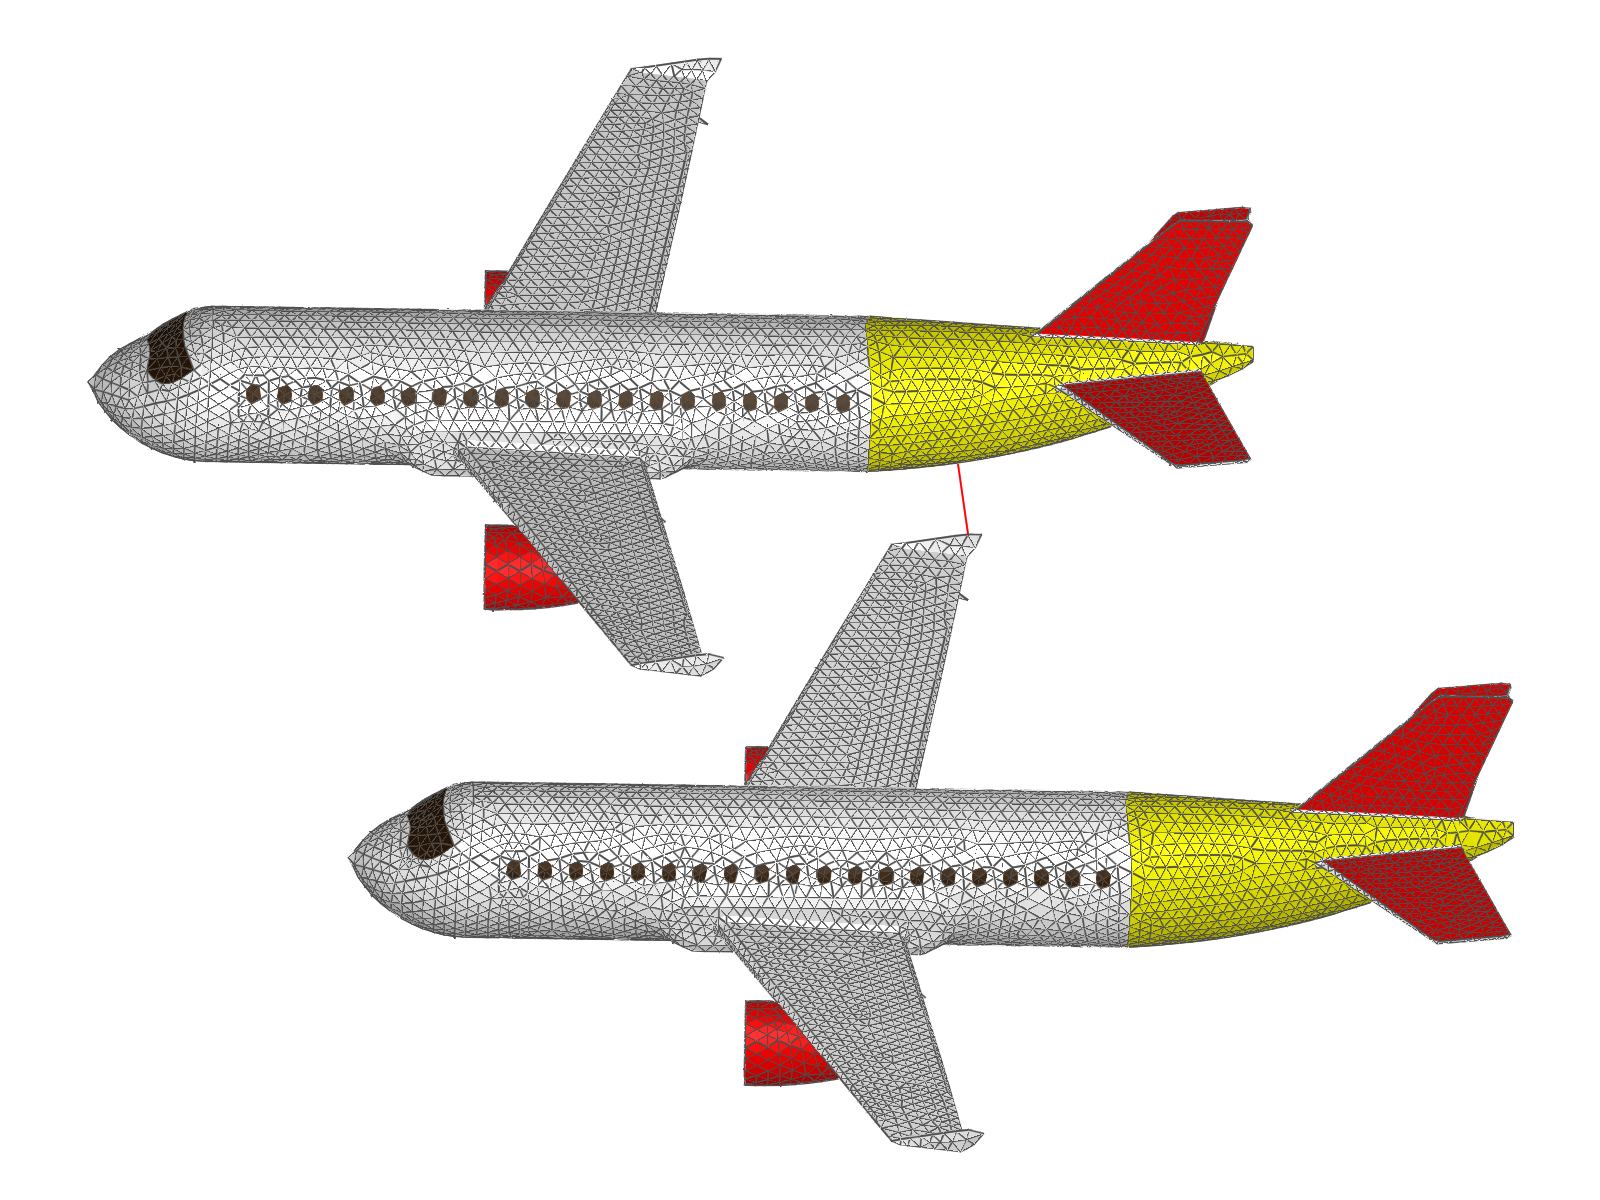
\includegraphics[width=0.9\textwidth]{testcase_scenes/airplanes_scene.png}
        \caption{Αεροπλάνα}
    \end{subfigure}
    \begin{subfigure}{0.49\textwidth}
        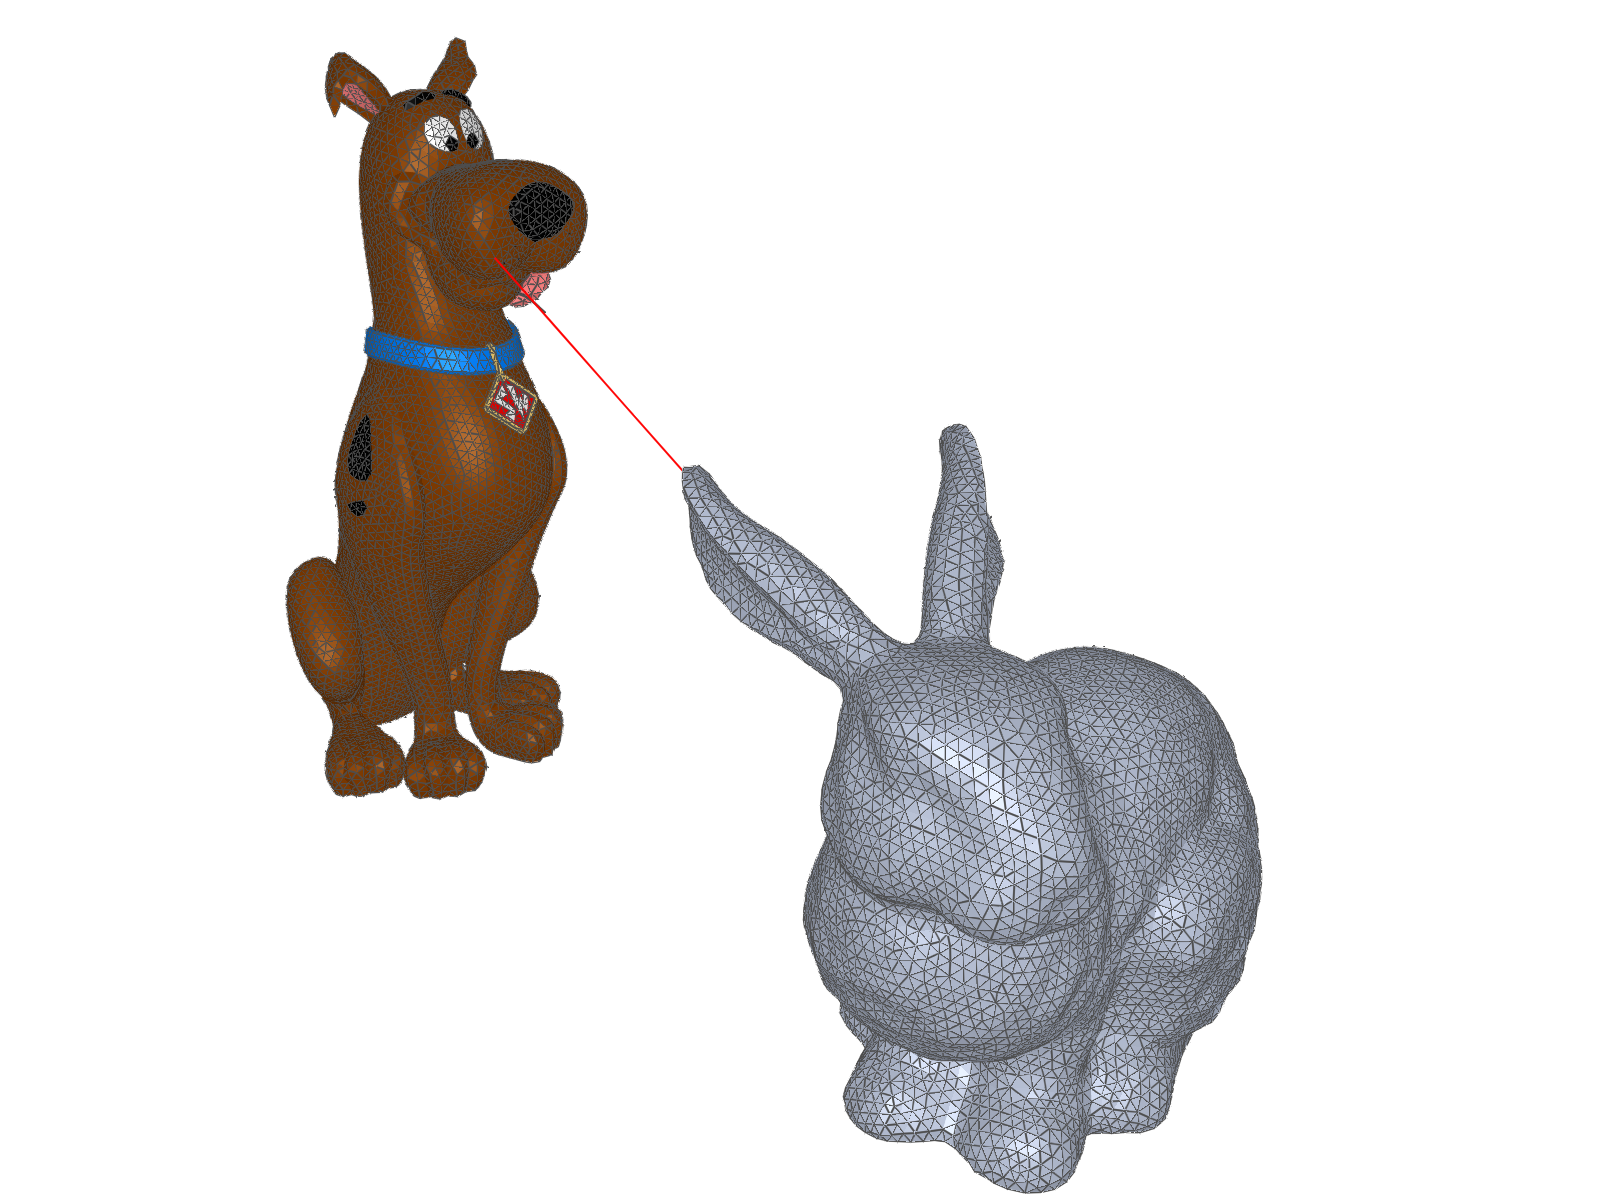
\includegraphics[width=0.9\textwidth]{testcase_scenes/scooby_w_bunny_scene.png}
        \caption{\tl{Scooby} με \tl{Stanford Bunny}}
    \end{subfigure}
    \begin{subfigure}{0.49\textwidth}
        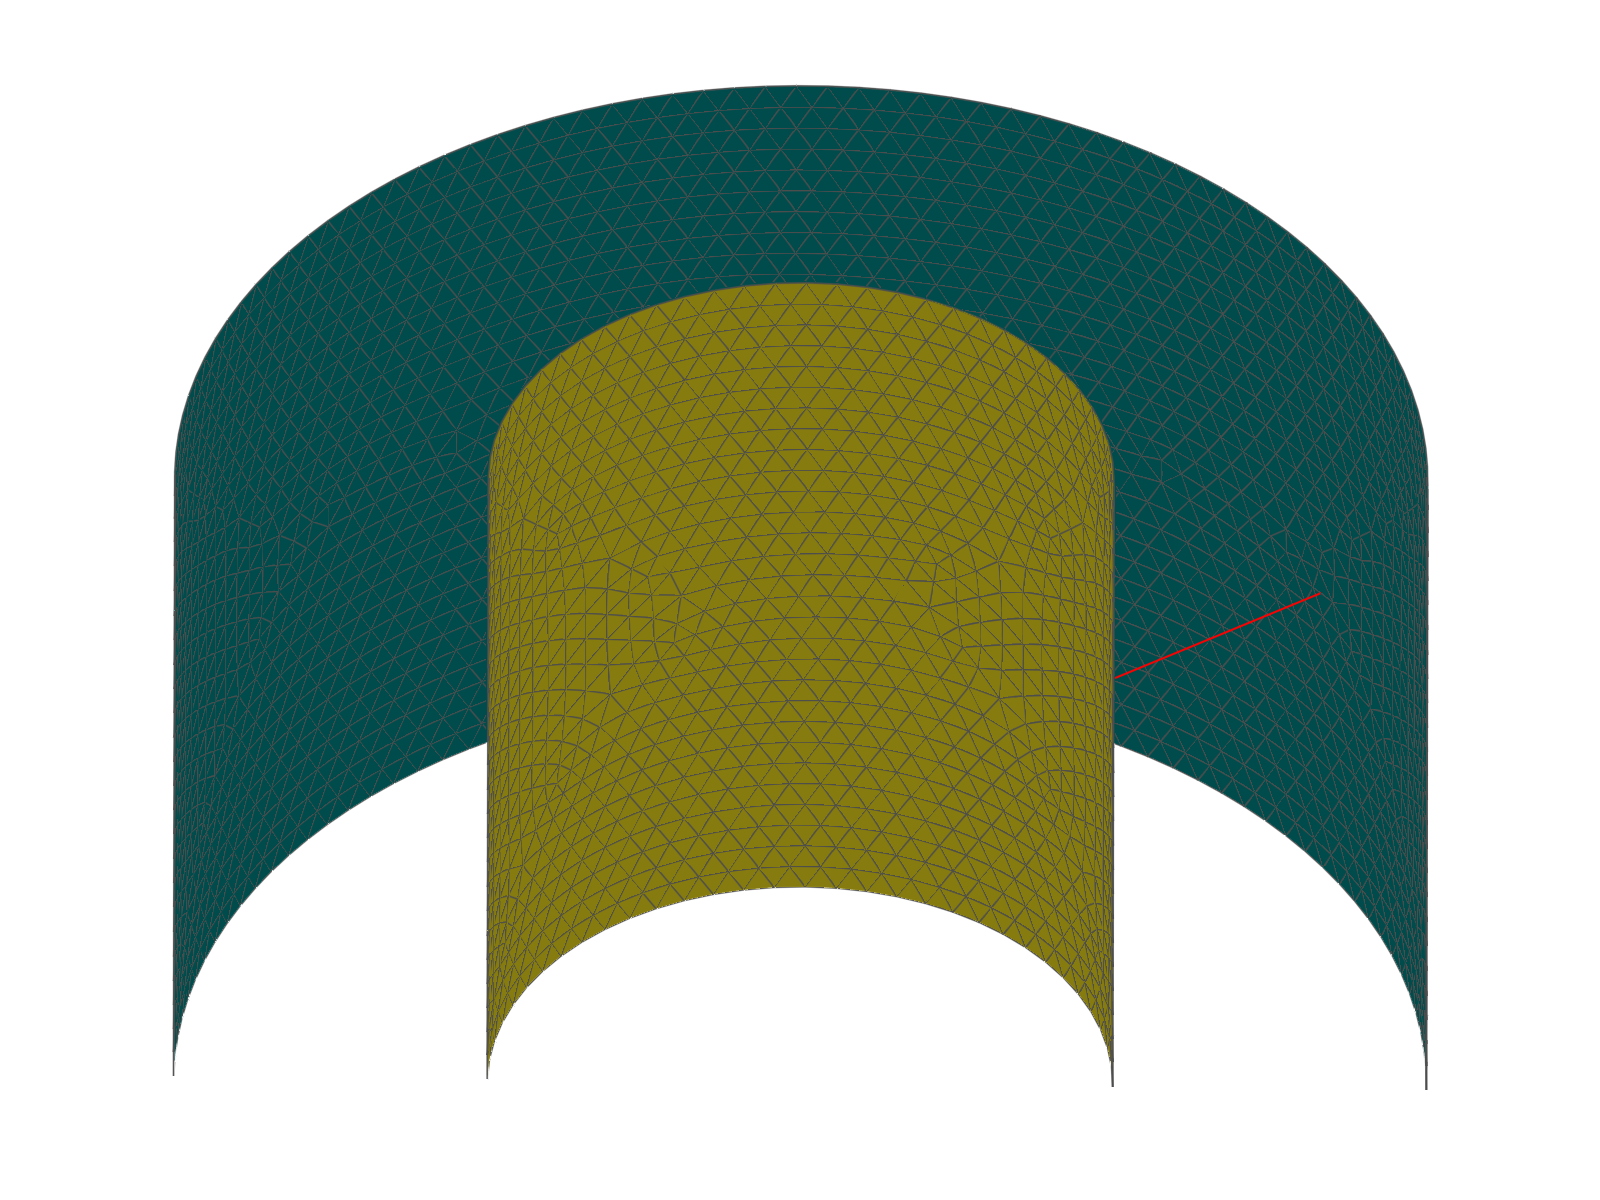
\includegraphics[width=0.9\textwidth]{testcase_scenes/cylinders_scene.png}
        \caption{Ομοαξονικοί ημι-κύλινδροι}
    \end{subfigure}
    \begin{subfigure}{0.49\textwidth}
        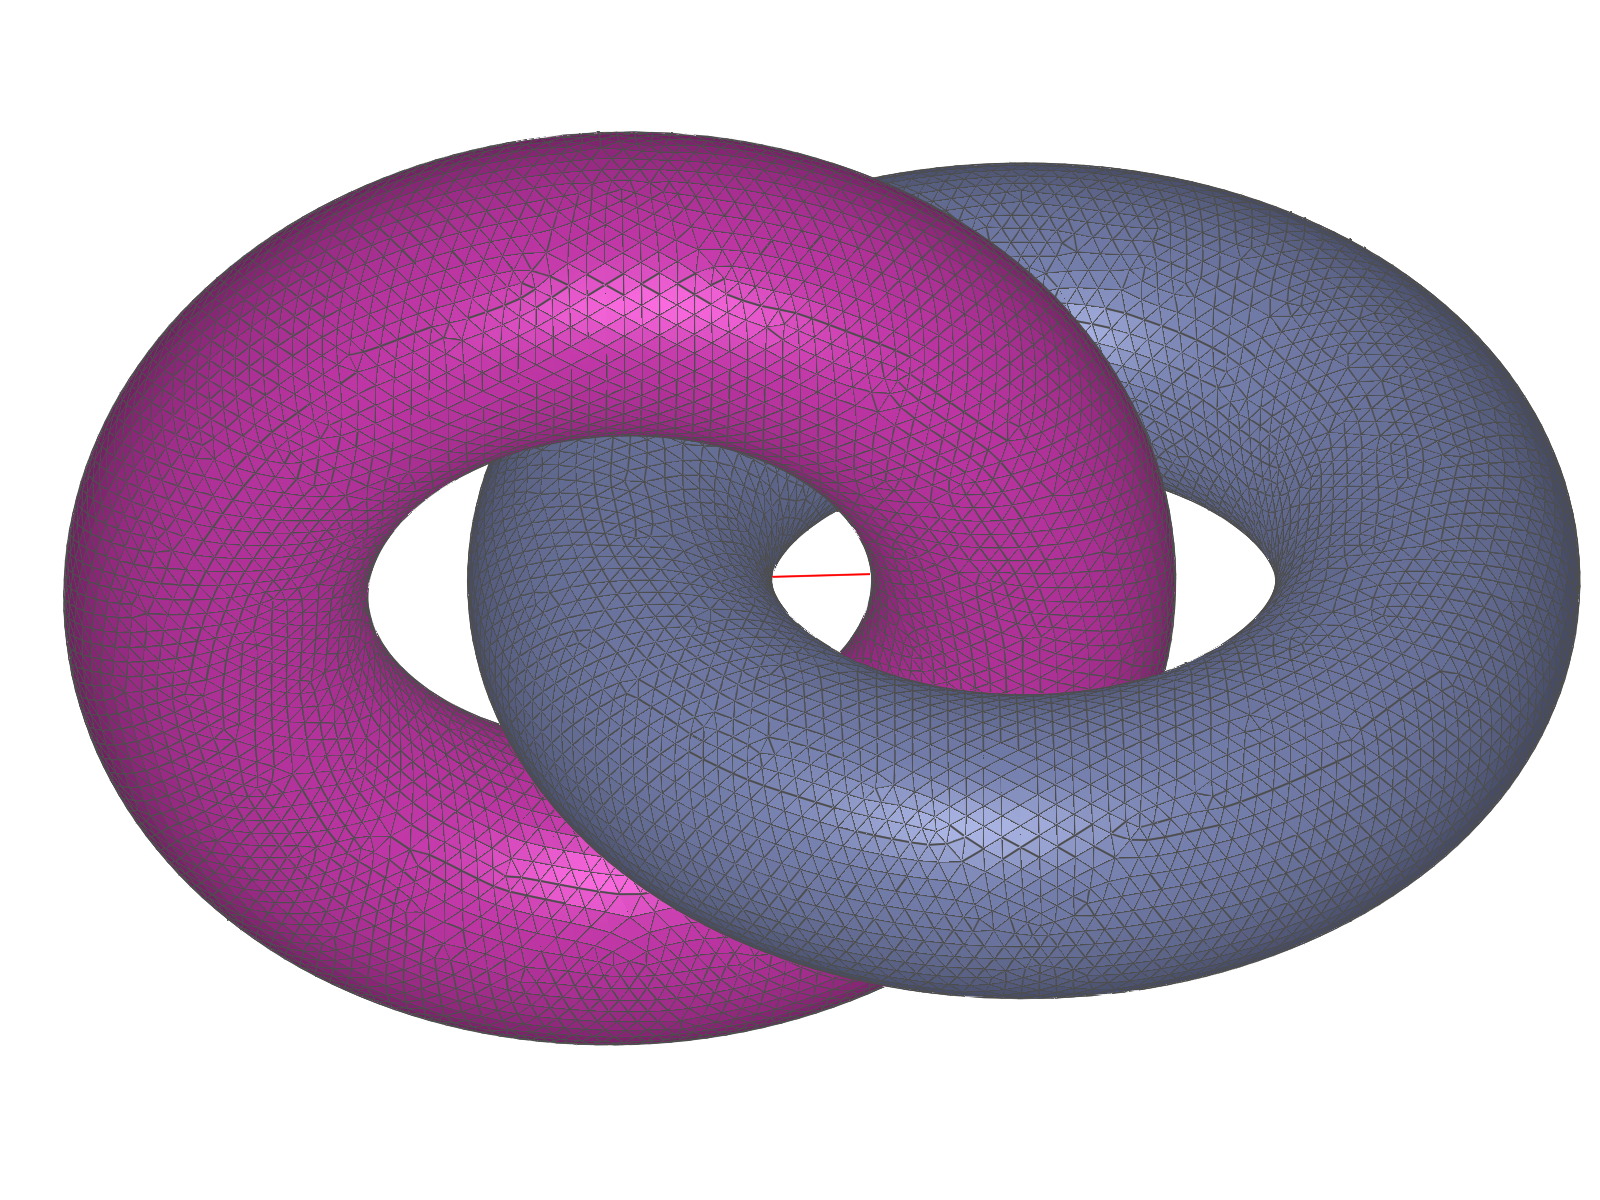
\includegraphics[width=0.9\textwidth]{testcase_scenes/chained_tori_scene.png}
        \caption{Αλυσιδωτοί Τόροι}
    \end{subfigure}
    \centering
    \begin{subfigure}{0.49\textwidth}
        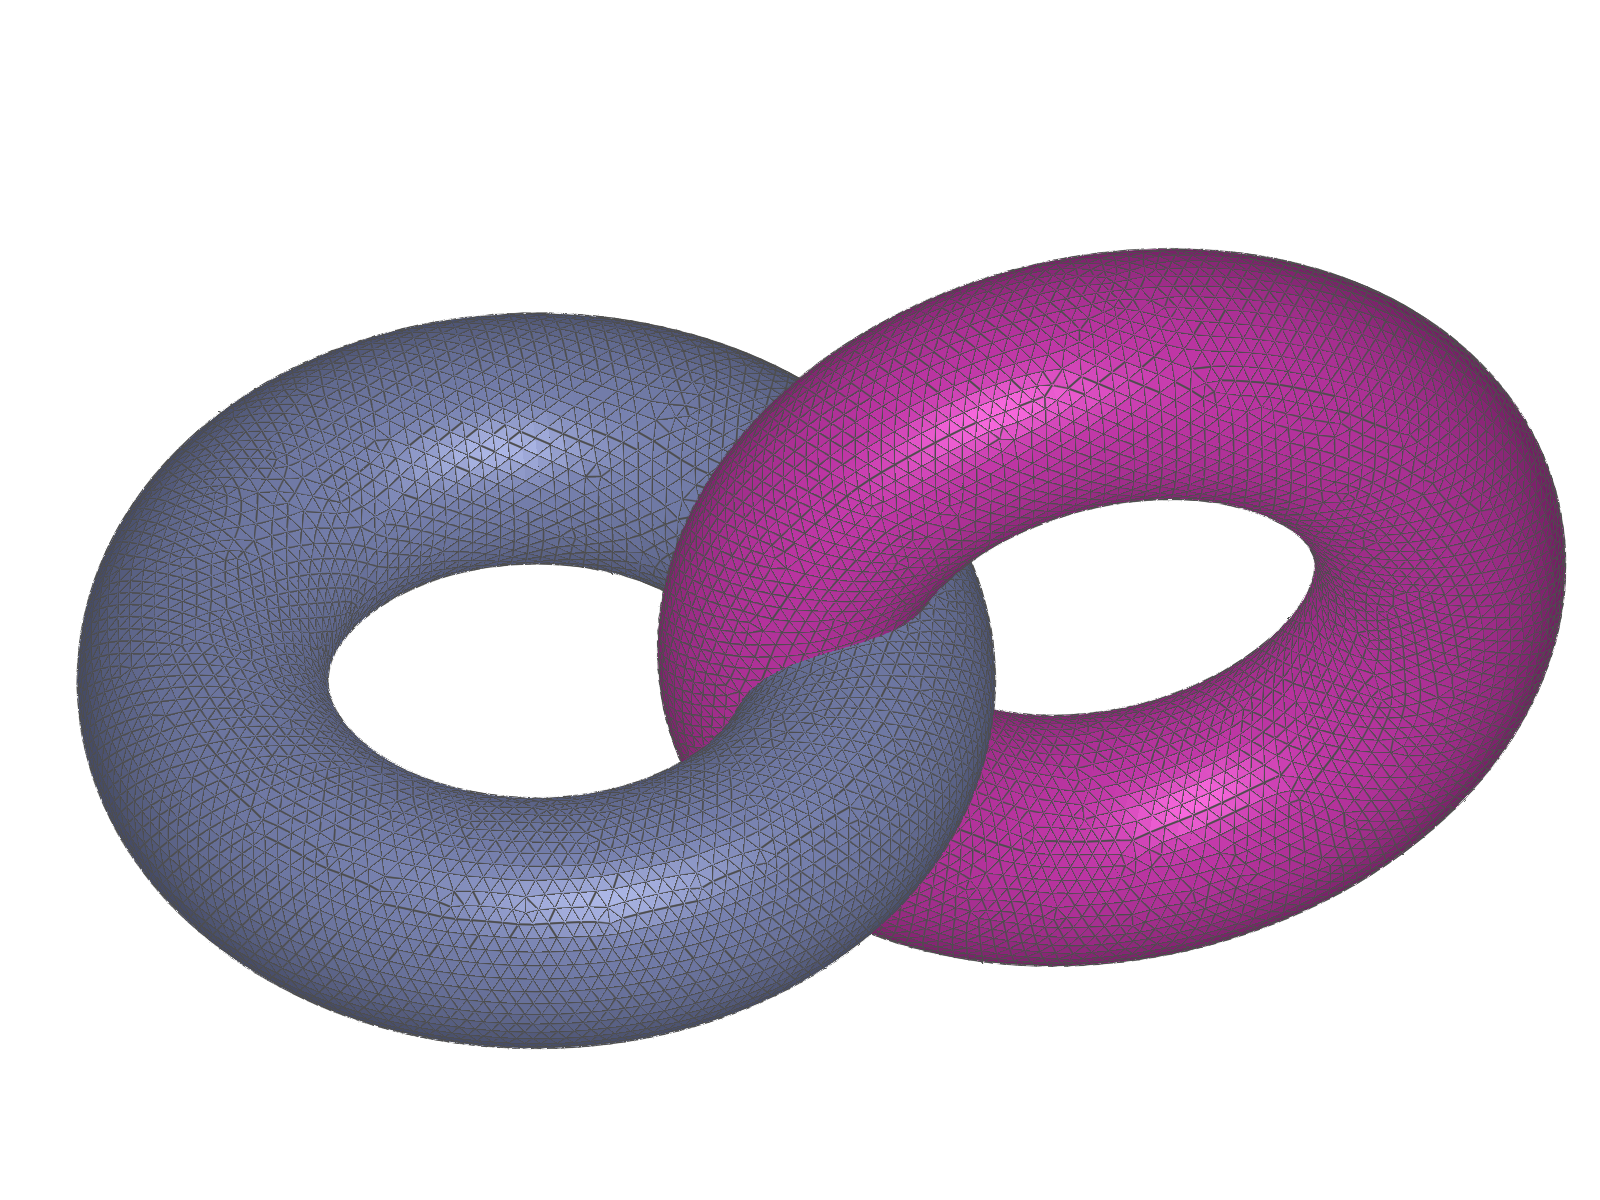
\includegraphics[width=0.9\textwidth]{testcase_scenes/colliding_tori_scene.png}
        \caption{Συγκρουόμενοι Τόροι}
    \end{subfigure}
    \caption[Οπτική αναπαράσταση των σεναρίων των πειραμάτων]{
        Οπτική αναπαράσταση των σεναρίων που χρησιμοποιήθηκαν για την 
        εκτέλεση των πειραμάτων της παρούσας εργασίας.
        Κάθε σενάριο αποτελείται από μία σκηνή με δύο αντικείμενα.  
        Το κόκκινο ευθύγραμμο τμήμα αναπαριστά την Ευκλείδεια απόσταση 
        των αντικειμένων.
    }
    \label{fig:scenarios_photos}
\end{figure}



\section{Χρόνος Κατασκευής του \tl{sKD-Tree}}
Στο σχήμα \ref{fig:build_time} παρουσιάζονται οι μετρήσεις του 
χρόνου κατασκευής του \tl{sKD-Tree} συναρτήσει του μεγέθους ενός 
τριγωνικού πλέγματος και του πλήθους των νημάτων (\tl{threads})
που χρησιμοποιήθηκαν.

\begin{figure}[h]
    \centering
    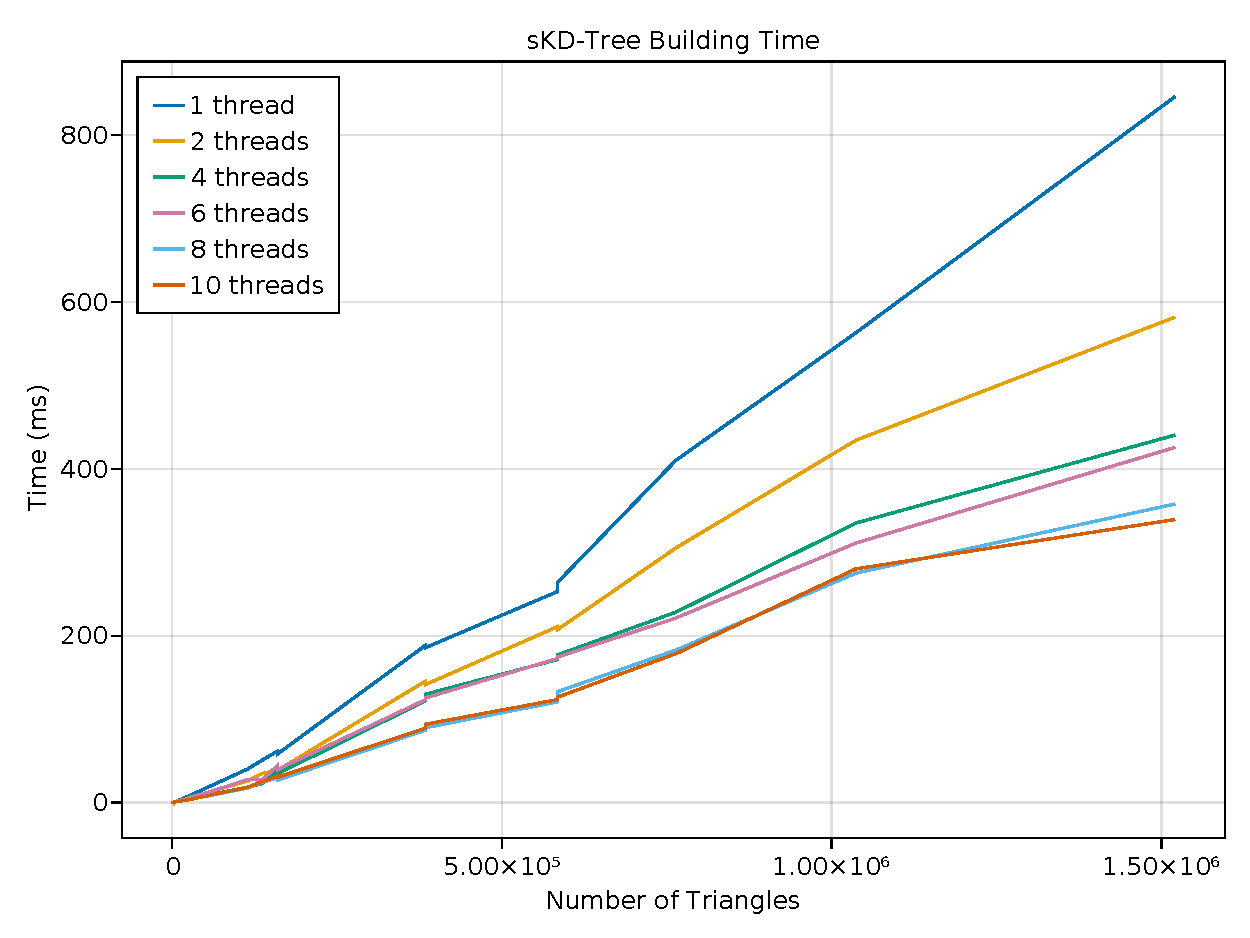
\includegraphics[width=0.6\textwidth]{build_time.pdf}
    \caption[Χρόνοι Κατασκευής του \tl{sKD-Tree}]{
        Χρόνος κατασκευής του \tl{sKD-Tree} συναρτήσει 
        του πλήθους των τριγώνων ενός πλέγματος.
    }
    \label{fig:build_time}
\end{figure}

\section{Πειράματα ανά Σενάριο}
Για κάθε ένα από τα παρακάτω σενάρια, παρουσιάζονται οι 
μετρήσεις για το κόστος αναζήτησης και το συνολικό χρόνο 
εκτέλεσης για την απάντηση ερωτημάτων απόστασης.
Στα διαγράμματα παρακάτω, γίνεται σύγκριση της επίδοσης των αλγορίθμων 
\ref{alg:queries_on_tree} και \ref{alg:search_on_two_trees}.

Το κόστος αναζήτησης υπολογίστηκε από τη μετρική κόστους 
που περιγράφεται στην ενότητα \ref{sec:cost_metric} 
μετρώντας τον αριθμό κλήσεων των ρουτινών 
\tl{\texttt{triangle\_distance()}} και \tl{\texttt{AABB\_distance()}}.
Σημειώνεται πως η καταμέτρηση των κλήσεων στις παραπάνω ρουτίνες 
πραγματοποιήθηκε για τη σειριακή εκτέλεση των αλγορίθμων, και συγκεκριμένα 
του αλγορίθμου \ref{alg:queries_on_tree}, αφού ο αλγόριθμος 
\ref{alg:search_on_two_trees} δεν είναι παράλληλος εκ κατασκευής.

Ο συνολικός χρόνος εκτέλεσης ερωτημάτων απόστασης περιλαμβάνει 
το χρόνο προεπεξεργασίας των δεδομένων και τον χρόνο αναζήτησης.
Η προεπεξεργασία των δεδομένων είναι η κατασκευή ενός ή δύο δέντρων 
ανάλογα με τον αλγόριθμο που χρησιμοποιείται.
Οι χρόνοι που παρουσιάζονται αντιστοιχούν σε πειράματα με χρήση 
ενός, τεσσάρων και οκτώ νημάτων επεξεργασίας.

Στο παράρτημα \ref{apndx:table_results} παρουσιάζονται πολλά από 
τα παρακάτω αποτελέσματα σε μορφή πινάκων, ώστε να γίνει μια πιο 
αναλυτική περιγραφή.

\subsection{Αεροπλάνα}

\begin{figure}[H]
    \centering
    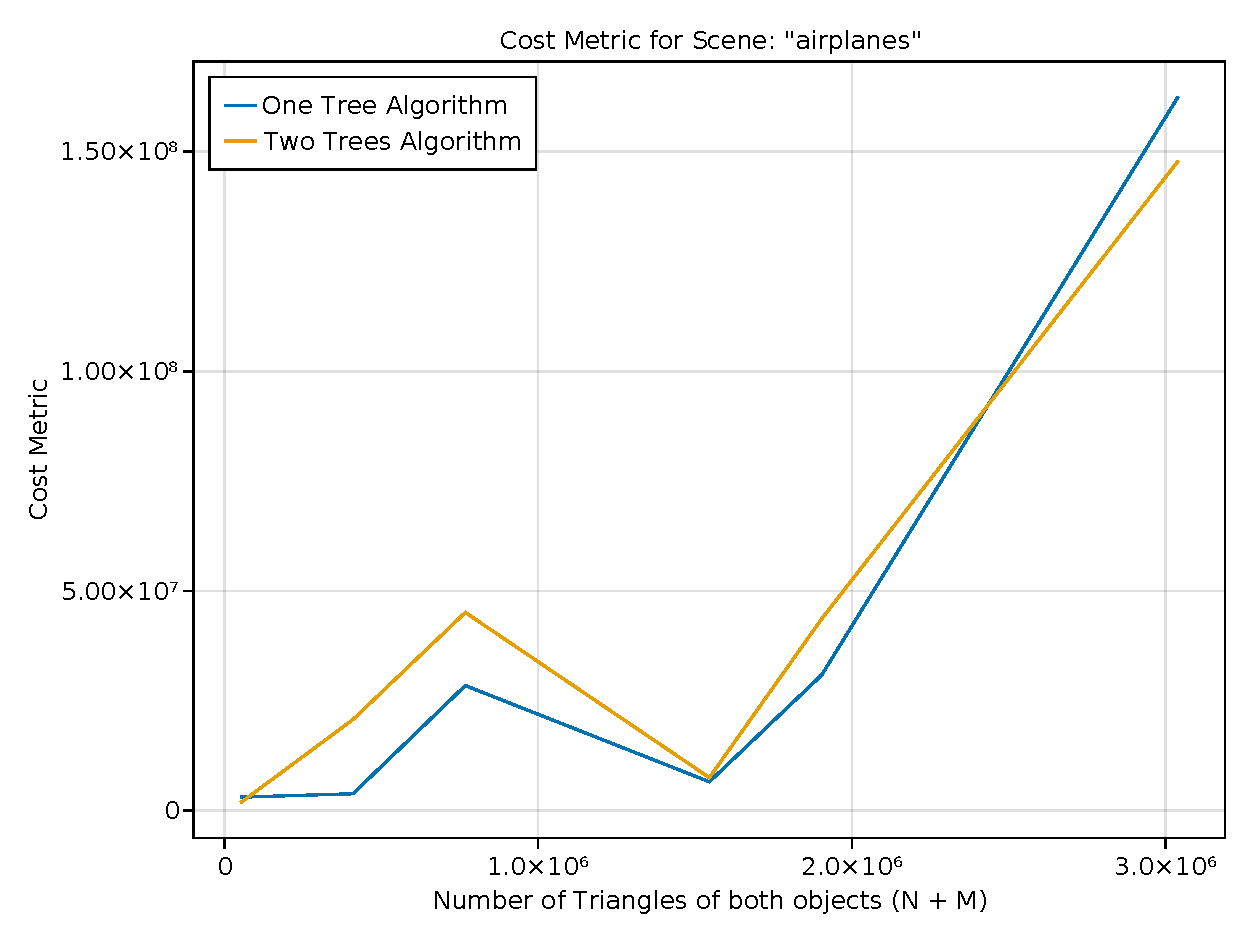
\includegraphics[width=0.6\textwidth]{cost_metric/airplanes_cost_metric.pdf}
    \caption[Κόστος Αναζήτησης για "αεροπλάνα"] {
        Κόστος αναζήτησης για τη σκηνή "αεροπλάνα" συναρτήσει 
        του μεγέθους των δύο μοντέλων.
    }
\end{figure}

\begin{figure}[H]
    \centering
    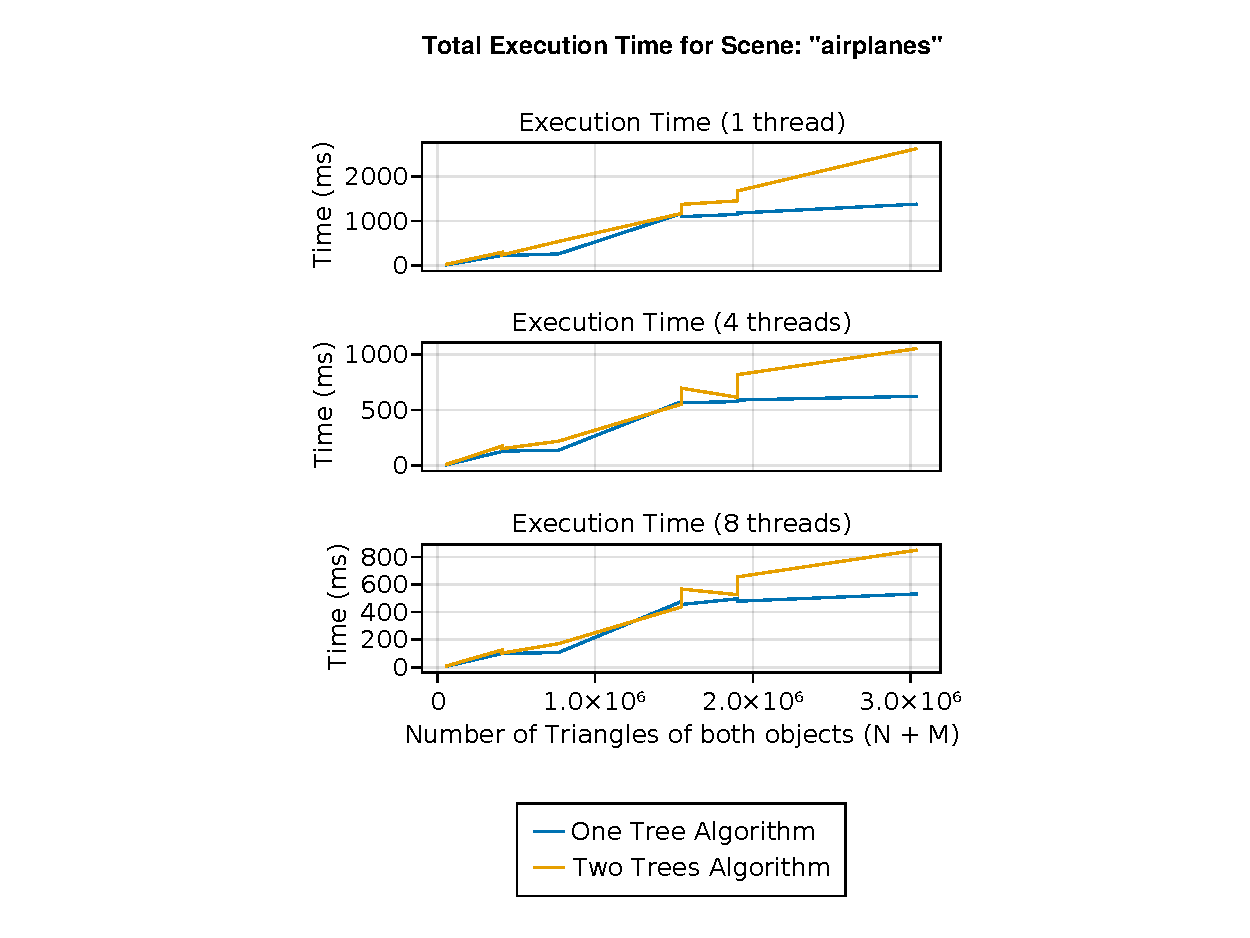
\includegraphics[width=1.0\textwidth]{execution_times/airplanes_exec_time.pdf}
    \caption[Συνολικός Χρόνος Εκτέλεσης για "αεροπλάνα"] {
        Συνολικός χρόνος εκτέλεσης ερωτήματος απόστασης 
        για τη σκηνή "αεροπλάνα" συναρτήσει του μεγέθους των δύο μοντέλων.
    }
\end{figure}

\subsection{\tl{Scooby} με \tl{Stanford Bunny}}
\begin{figure}[H]
    \centering
    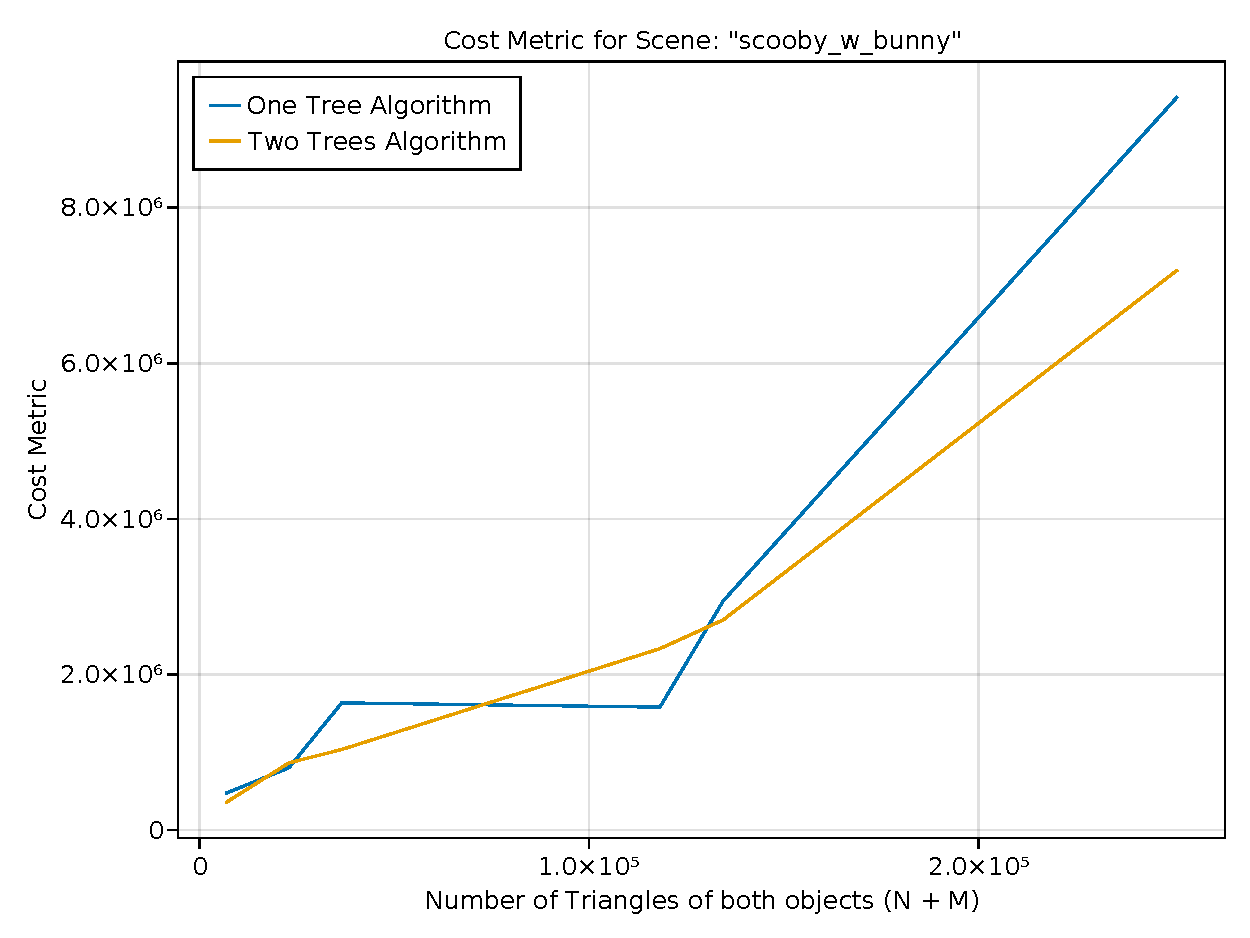
\includegraphics[width=0.6\textwidth]{cost_metric/scooby_w_bunny_cost_metric.pdf}
    \caption[Κόστος Αναζήτησης για "\tl{Scooby} με \tl{Stanford Bunny}"] {
        Κόστος αναζήτησης για τη σκηνή "\tl{Scooby} με \tl{Stanford Bunny}" συναρτήσει 
        του μεγέθους των δύο μοντέλων.
    }
\end{figure}

\begin{figure}[H]
    \centering
    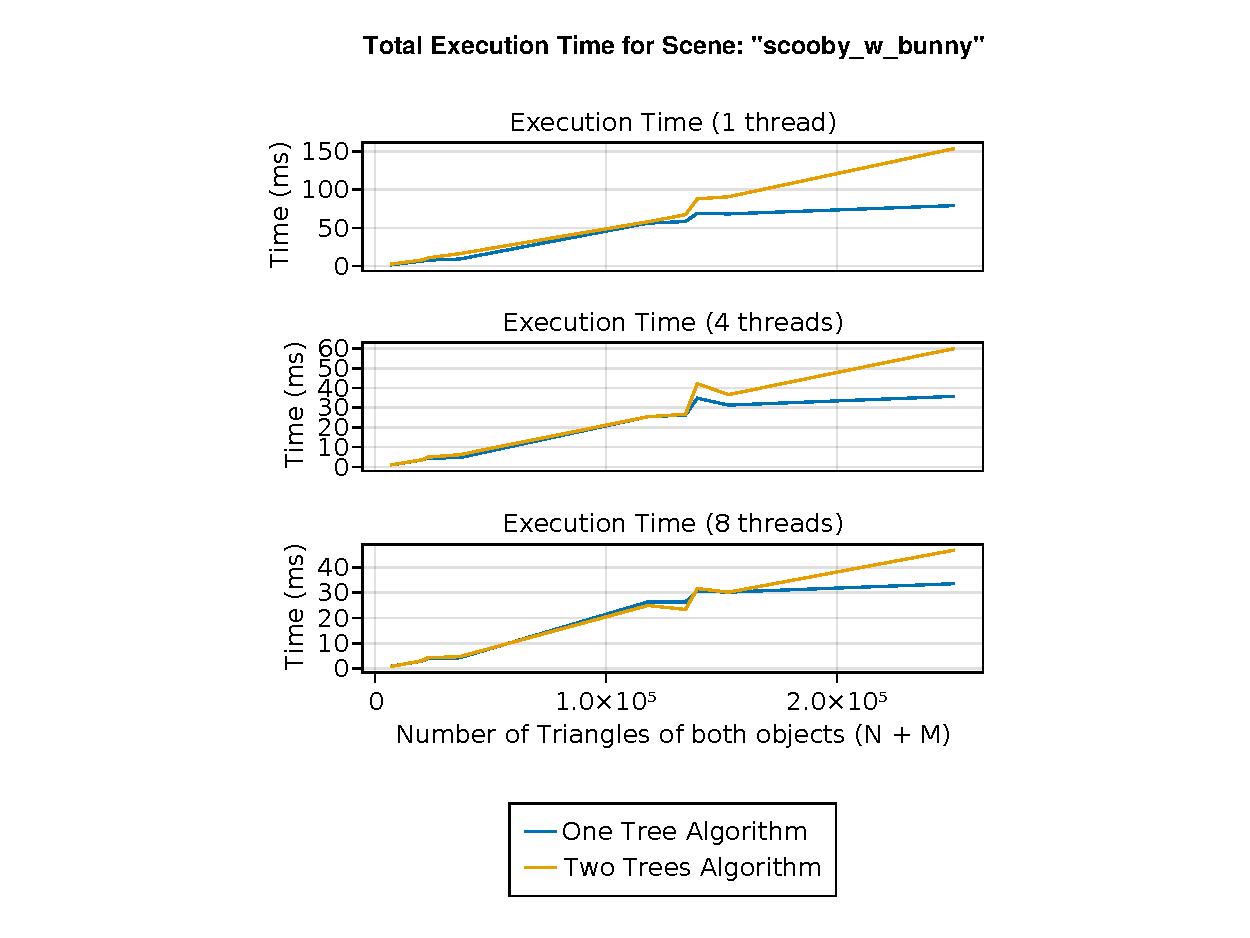
\includegraphics[width=1.0\textwidth]{execution_times/scooby_w_bunny_exec_time.pdf}
    \caption[Συνολικός Χρόνος Εκτέλεσης για "\tl{Scooby} με \tl{Stanford Bunny}"] {
        Συνολικός χρόνος εκτέλεσης ερωτήματος απόστασης 
        για τη σκηνή "\tl{Scooby} με \tl{Stanford Bunny}" συναρτήσει του μεγέθους των δύο μοντέλων.
    }
\end{figure}


\subsection{Ομοαξονικοί Κύλινδροι}
\begin{figure}[H]
    \centering
    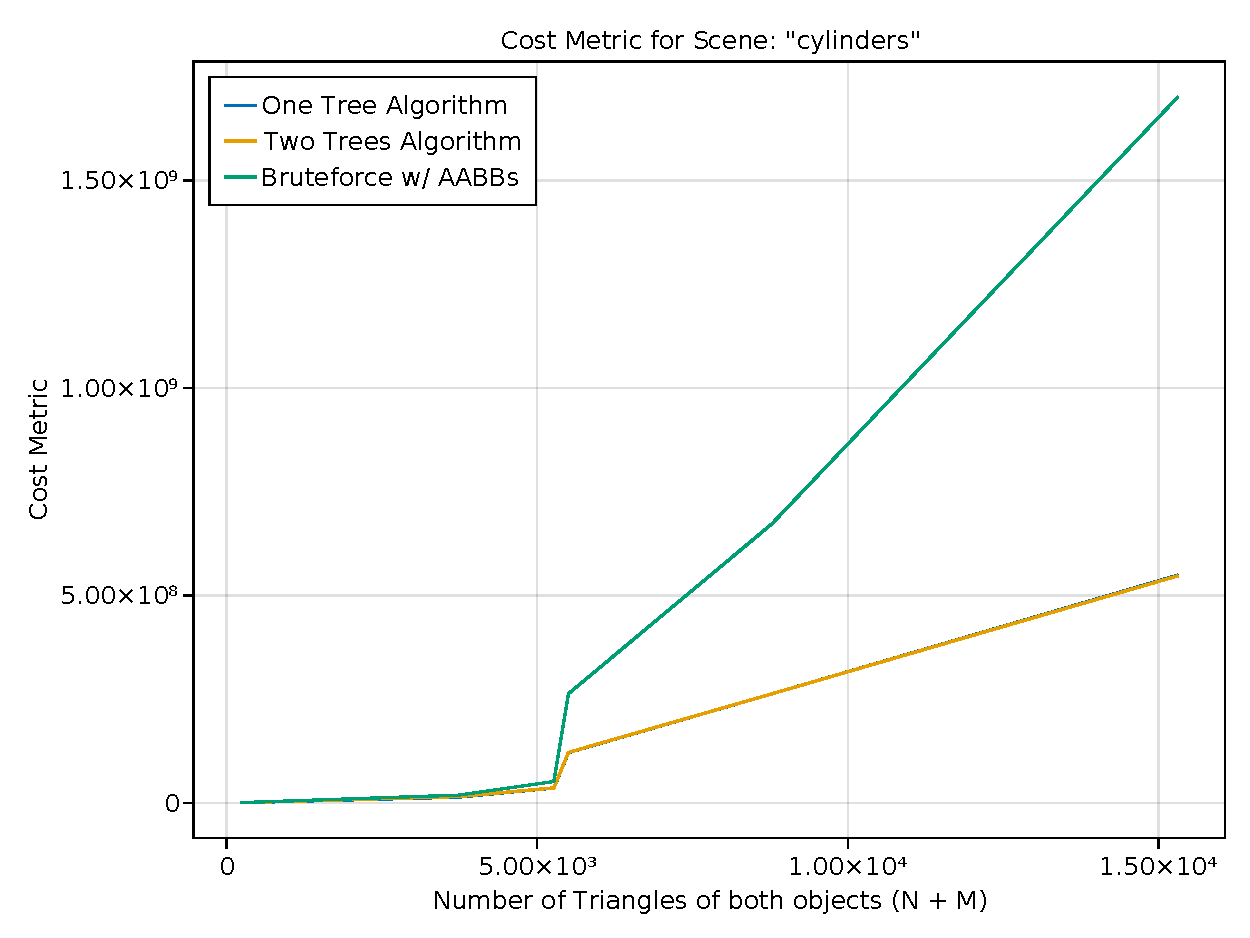
\includegraphics[width=0.6\textwidth]{cost_metric/cylinders_cost_metric.pdf}
    \caption[Κόστος Αναζήτησης για "ομοαξονικοί κύλινδροι"] {
        Κόστος αναζήτησης για τη σκηνή "ομοαξονικοί κύλινδροι" συναρτήσει 
        του μεγέθους των δύο μοντέλων.
    }
\end{figure}

\begin{figure}[H]
    \centering
    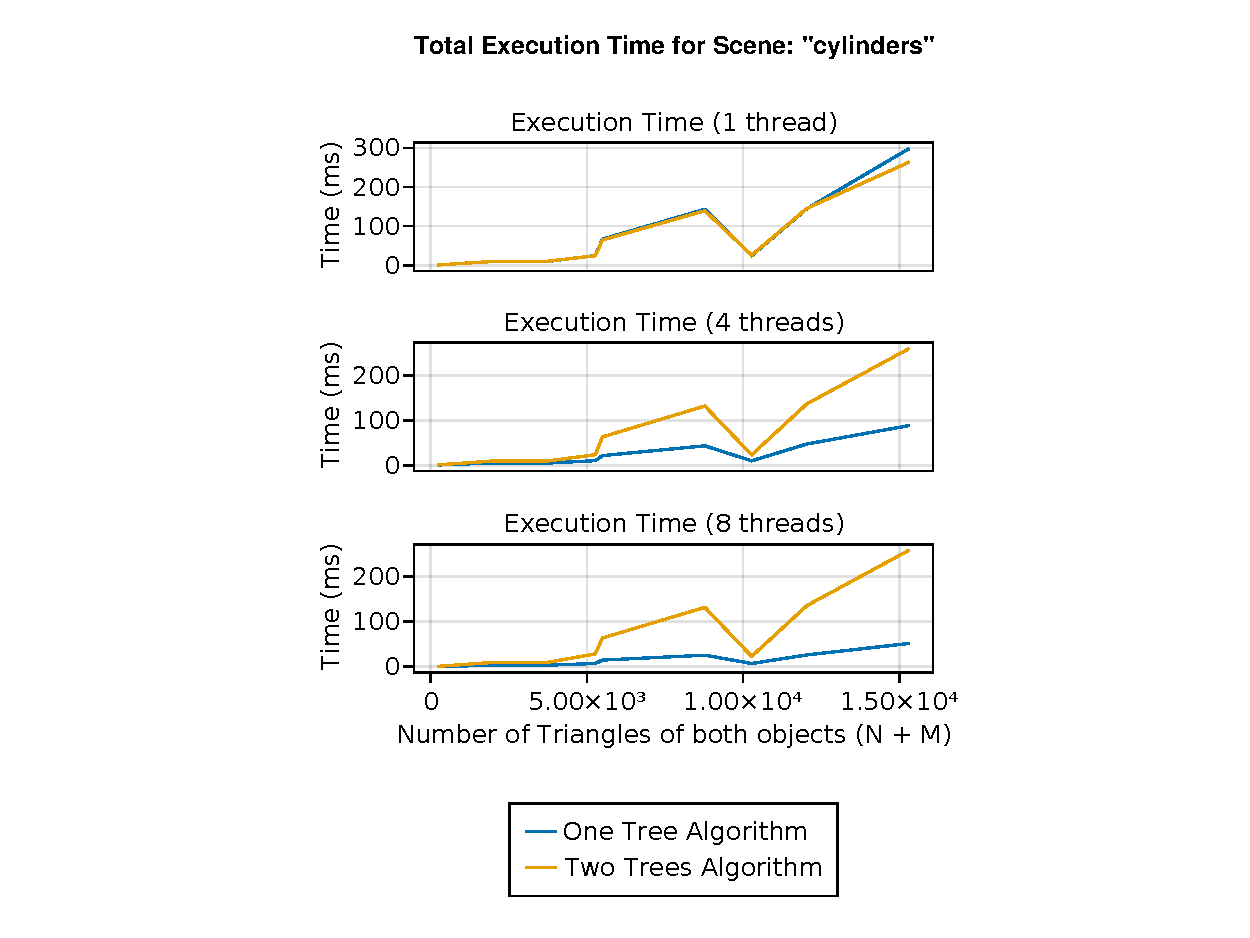
\includegraphics[width=1.0\textwidth]{execution_times/cylinders_exec_time.pdf}
    \caption[Συνολικός Χρόνος Εκτέλεσης για "ομοαξονικοί κύλινδροι"] {
        Συνολικός χρόνος εκτέλεσης ερωτήματος απόστασης 
        για τη σκηνή "ομοαξονικοί κύλινδροι" συναρτήσει του μεγέθους των δύο μοντέλων.
    }
\end{figure}


\subsection{Αλυσιδωτοί Τόροι}
\begin{figure}[H]
    \centering
    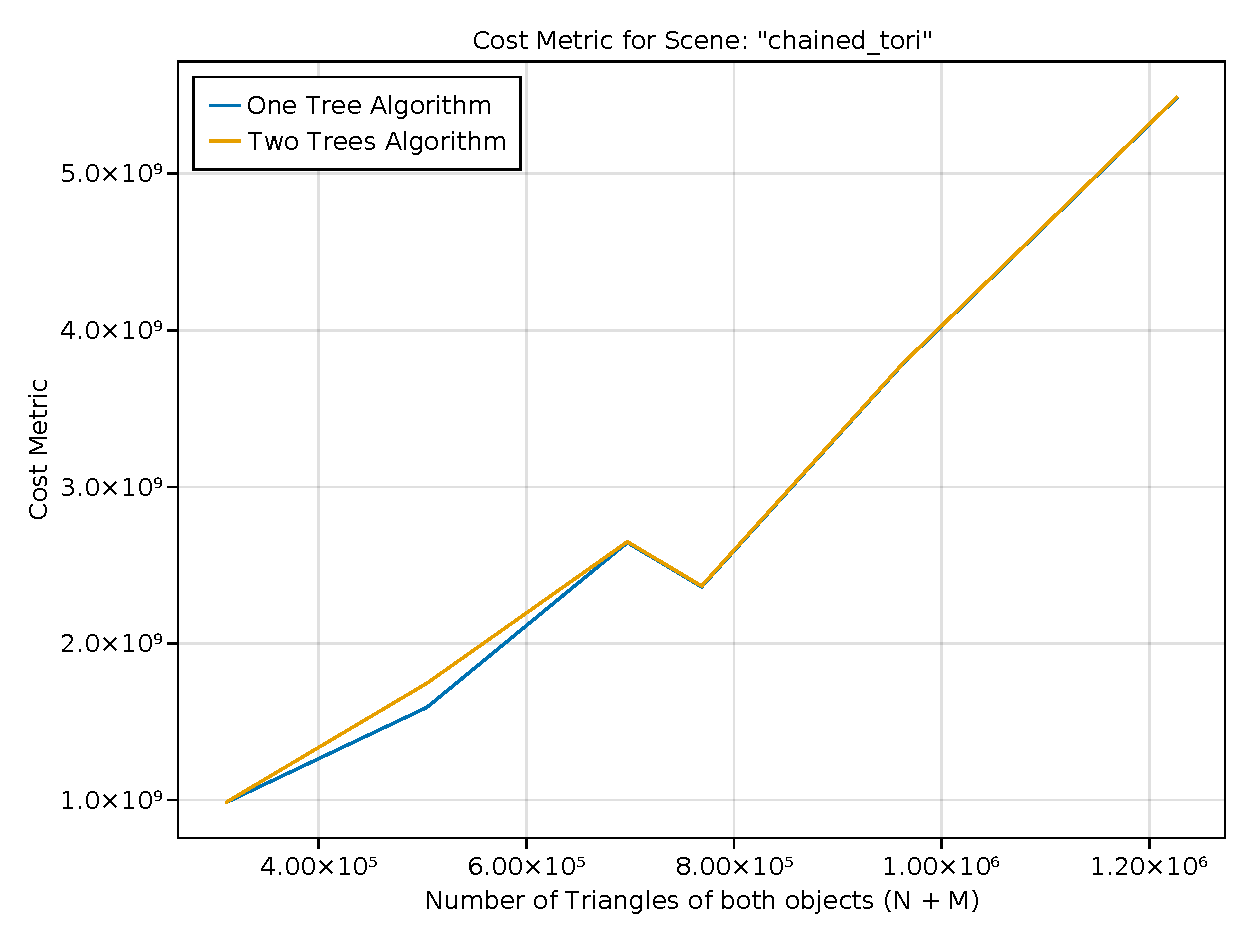
\includegraphics[width=0.6\textwidth]{cost_metric/chained_tori_cost_metric.pdf}
    \caption[Κόστος Αναζήτησης για "αλυσιδωτοί τόροι"] {
        Κόστος αναζήτησης για τη σκηνή "αλυσιδωτοί τόροι" συναρτήσει 
        του μεγέθους των δύο μοντέλων.
    }
\end{figure}

\begin{figure}[H]
    \centering
    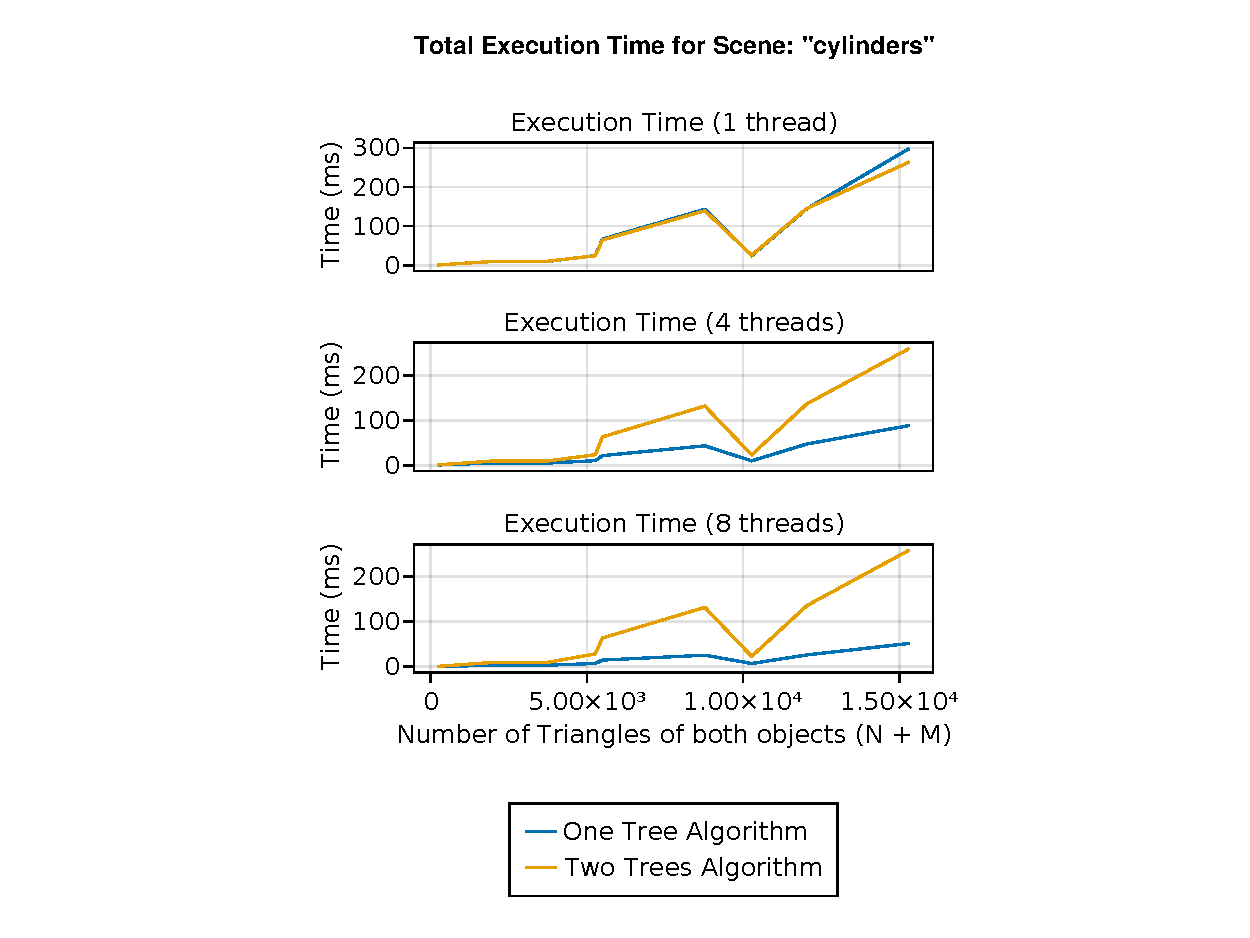
\includegraphics[width=1.0\textwidth]{execution_times/cylinders_exec_time.pdf}
    \caption[Συνολικός Χρόνος Εκτέλεσης για "ομοαξονικοί κύλινδροι"] {
        Συνολικός χρόνος εκτέλεσης ερωτήματος απόστασης 
        για τη σκηνή "ομοαξονικοί κύλινδροι" συναρτήσει του μεγέθους των δύο μοντέλων.
    }
\end{figure}

\subsection{Συγκρουόμενοι Τόροι}
\begin{figure}[H]
    \centering
    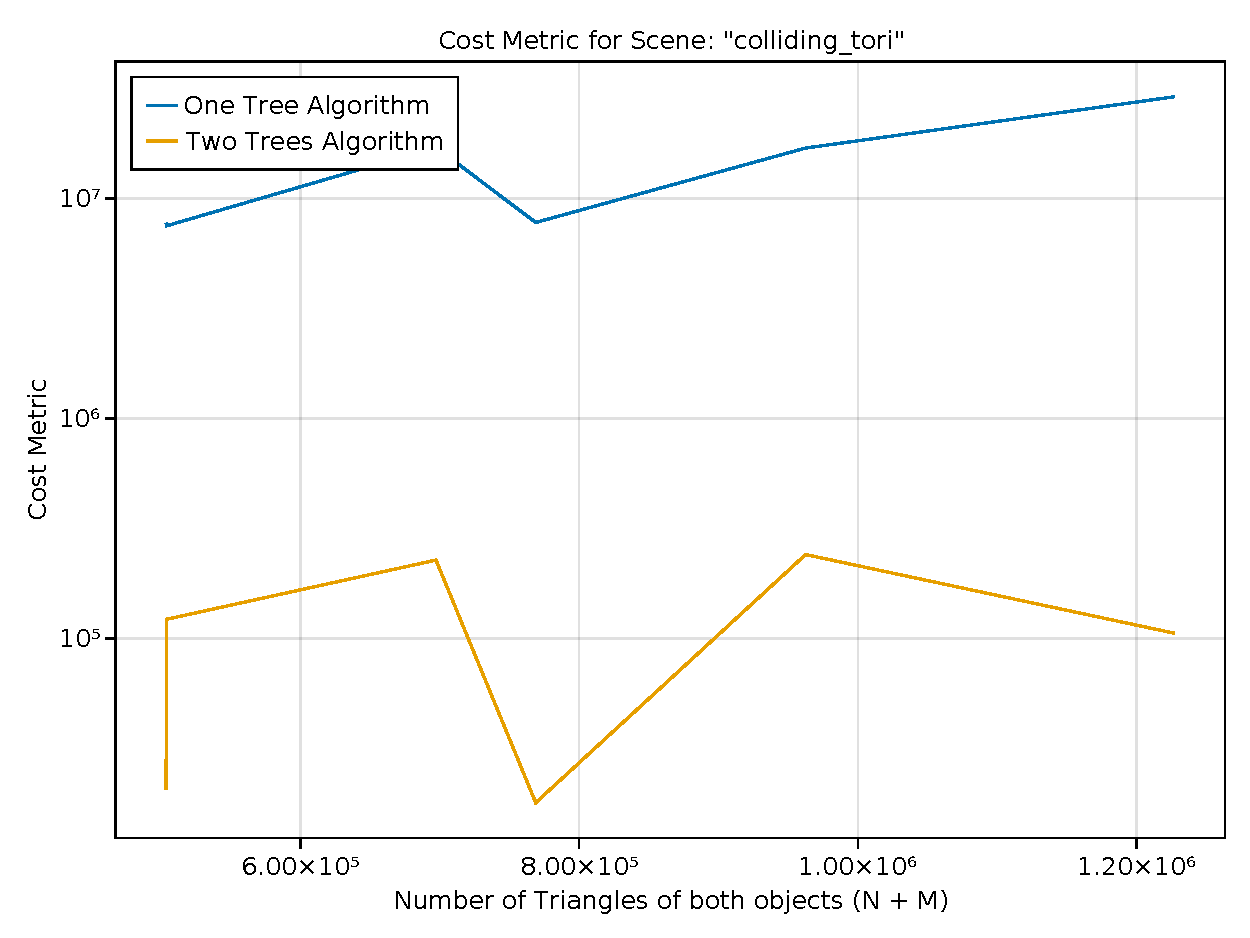
\includegraphics[width=0.6\textwidth]{cost_metric/colliding_tori_cost_metric.pdf}
    \caption[Κόστος Αναζήτησης για "συγκρουόμενοι τόροι"] {
        Κόστος αναζήτησης για τη σκηνή "συγκρουόμενοι τόροι" συναρτήσει 
        του μεγέθους των δύο μοντέλων.
    }
\end{figure}

\begin{figure}[H]
    \centering
    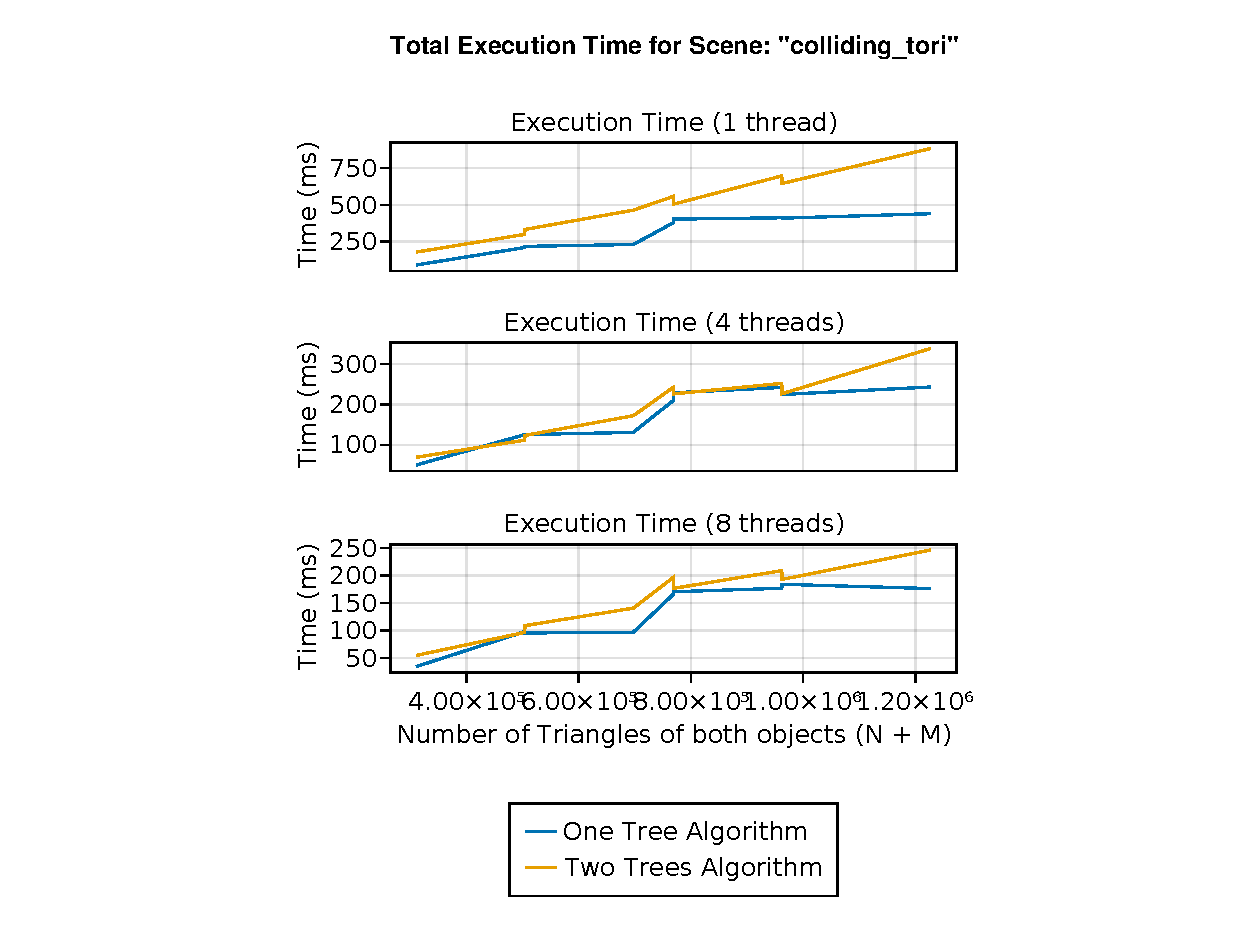
\includegraphics[width=1.0\textwidth]{execution_times/colliding_tori_exec_time.pdf}
    \caption[Συνολικός Χρόνος Εκτέλεσης για "συγκρουόμενοι τόροι"] {
        Συνολικός χρόνος εκτέλεσης ερωτήματος απόστασης 
        για τη σκηνή "συγκρουόμενοι τόροι" συναρτήσει του μεγέθους των δύο μοντέλων.
    }
\end{figure}


\section{Σχέση Απόστασης - Κόστους Αναζήτησης}
Για το πείραμα αυτό επιλέχθηκαν τα αντικείμενα της σκηνής 
"Αεροπλάνα" με περίπου $1.5 * 10^6$ τρίγωνα το καθένα.
Η αρχική θέση των αντικειμένων είναι αυτή που απεικονίζεται 
στην εικόνα \ref{fig:scenarios_photos}.
Έπειτα το ένα αεροπλάνο μετακινείται 
προς μια κατεύθυνση τέτοια ώστε να απομακρύνεται 
από το άλλο αεροπλάνο.

Στην εικόνα \ref{fig:cost_metric_vs_distance} 
σχεδιάζεται το κόστος αναζήτησης συναρτήσει της 
κανονικοποιημένης απόστασης των αντικειμένων, 
ενώ στην εικόνα \ref{fig:search_time_vs_distance} 
παρουσιάζεται ο χρόνος αναζήτησης (μόνο) συναρτήσει 
της κανονικοποιημένης απόστασης. 
Η απόσταση είναι κανονικοποιημένη και ίση με 
$\frac{dist}{diagonal}$, όπου $dist$ η πραγματική 
απόσταση των αντικειμένων και $diagonal$ το μήκος 
της διαγωνίου του \tl{AABB} του αεροπλάνου.


\begin{figure}[H]
    \centering
    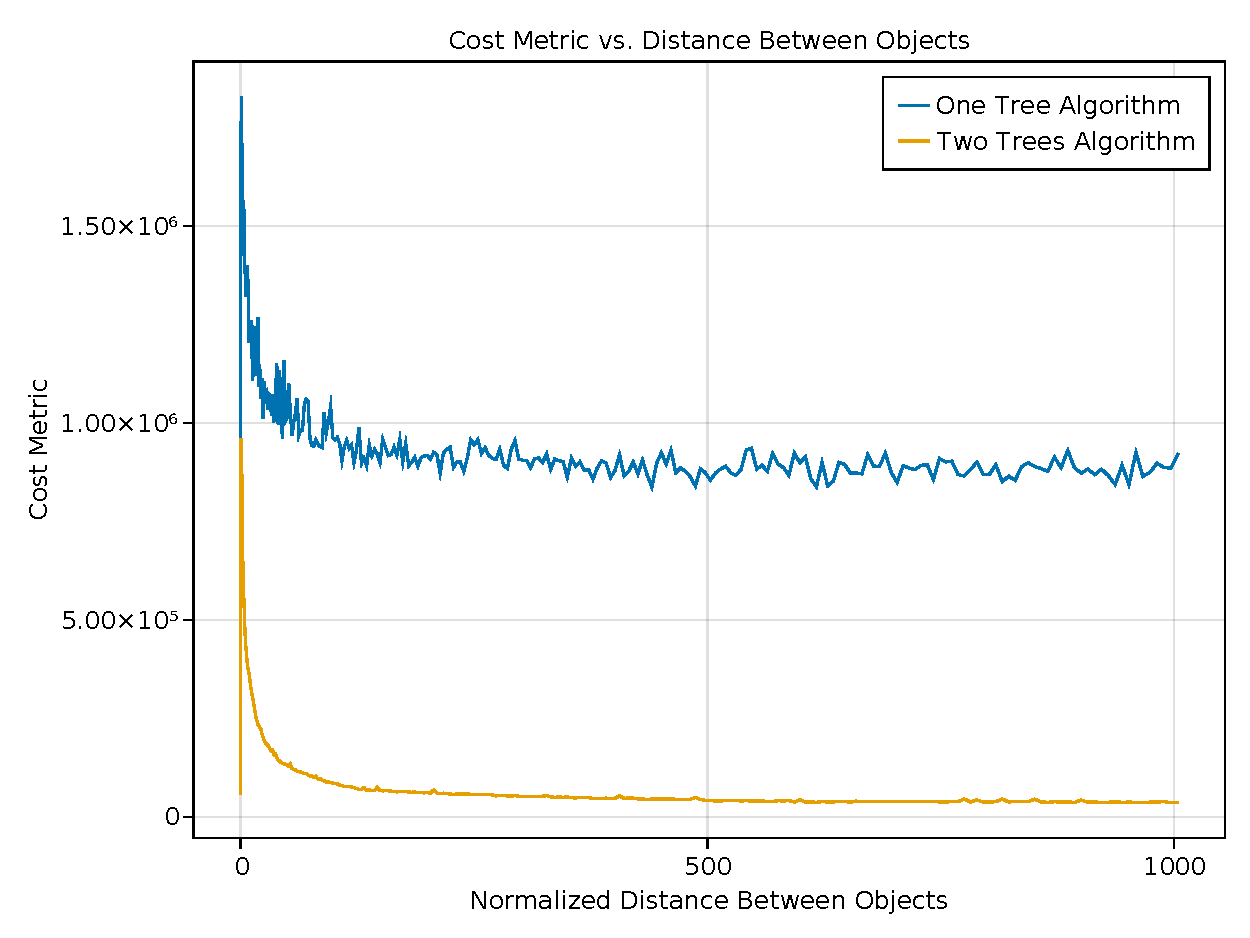
\includegraphics[width=0.6\textwidth]{cost_vs_distance.pdf}
    \caption[Κόστος Αναζήτησης Συναρτήσει της Απόστασης"] {
        Κόστος αναζήτησης συναρτήσει της απόστασης.
        Τα αντικείμενα ανήκουν στη σκηνή "αεροπλάνα".
    }
    \label{fig:cost_metric_vs_distance}
\end{figure}

\begin{figure}[H]
    \centering
    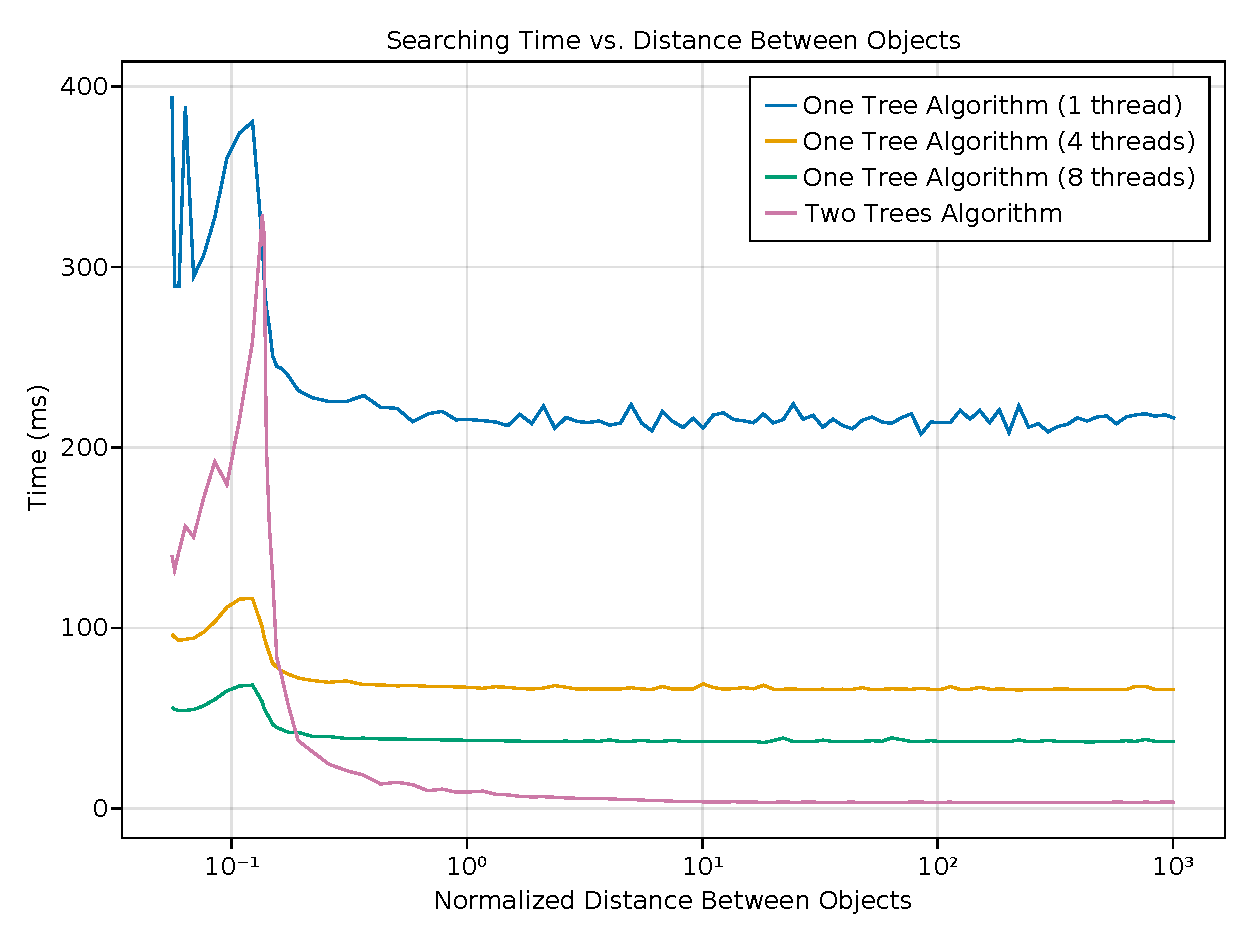
\includegraphics[width=0.6\textwidth]{search_time_vs_distance.pdf}
    \caption[Χρόνος Αναζήτησης Συναρτήσει της Απόστασης"] {
        Χρόνος αναζήτησης συναρτήσει της απόστασης.
        Τα αντικείμενα ανήκουν στη σκηνή "αεροπλάνα".
        \textit{Σημείωση}: Ο αλγόριθμος που χρησιμοποιεί δύο \tl{sKD-Trees} δεν 
        είναι παράλληλος.
    }
    \label{fig:search_time_vs_distance}
\end{figure}




% να προσθέσω ποσοστά χρόνου αναζήτησης/κατασκευής
